% Created 2016-11-27 Sun 17:39
% Intended LaTeX compiler: pdflatex
\documentclass[11pt]{article}
\usepackage[utf8]{inputenc}
\usepackage[T1]{fontenc}
\usepackage{graphicx}
\usepackage{grffile}
\usepackage{longtable}
\usepackage{wrapfig}
\usepackage{rotating}
\usepackage[normalem]{ulem}
\usepackage{amsmath}
\usepackage{textcomp}
\usepackage{amssymb}
\usepackage{capt-of}
\usepackage{hyperref}
\author{killian}
\date{\today}
\title{CS4032 Protocol}
\hypersetup{
 pdfauthor={killian},
 pdftitle={CS4032 Protocol},
 pdfkeywords={},
 pdfsubject={},
 pdfcreator={Emacs 24.5.1 (Org mode 9.0.1)}, 
 pdflang={English}}
\begin{document}

\maketitle
\tableofcontents


\section{General Protocol}
\label{sec:org445e5cf}

\subsection{Propagation of certs}
\label{sec:orgb58201d}
\#\#ile:certificate\(_{\text{propogation.png}}\)]]

All connecting servers must report their public keys to the auth server. The auth server can only trust the identity of the server providing the cert by encrpyting this channel with a pre shared key.
The server admin manages the sharing of this key.


\subsection{TLS and server trust model}
\label{sec:orgc450b71}
\#\#\#\#iletls\(_{\text{server}}_{\text{trust.png}}\)]]

All comms are over TLS. If the admin sets everything up correctly, all servers will have the self signed certs of all the other servers, or at least the ones which they will communicate with.
If a user connects to the auth server, they must decide whether to trust the auth servers cert. If they do, the auth server can vouch for the validity of the public keys for all the other servers. Therefore,
the user can now communicate with encrypted and authenticated comms with integrity. 
\subsection{User auth}
\label{sec:org0f2d183}
\begin{center}
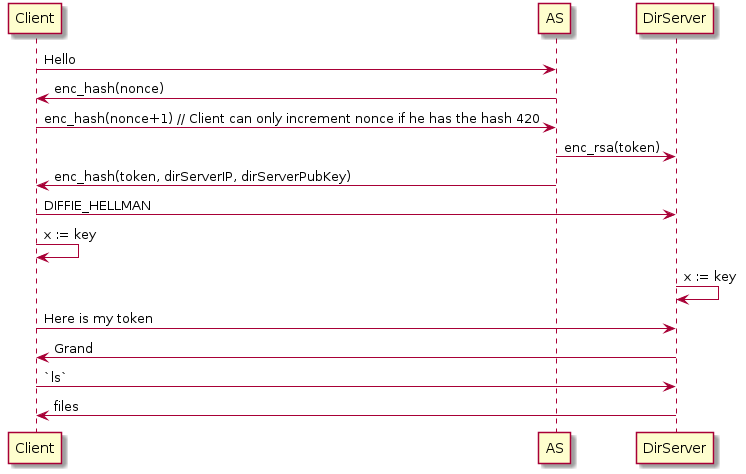
\includegraphics[width=.9\linewidth]{security.png}
\end{center}

After TLS is setup to the auth server, all we need worry about is authing the user. User hashes their password, send that hash and user\(_{\text{id}}\) to the auth server. Auth server then looks up the data and can verify the user.
The auth server generates a random token, and distributes this to all the other servers with a specified expiry time. The user also gets this token. Very simply, if a user wants to connect to a server, they
provide the token thereby proving that they have authed with the auth server.

\subsection{Get file from server}
\label{sec:org3f08346}


\begin{center}
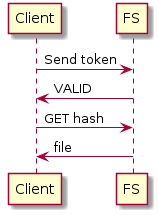
\includegraphics[width=.9\linewidth]{get_file.png}
\end{center}

\subsection{Put file from server}
\label{sec:orgeae1245}
\begin{center}
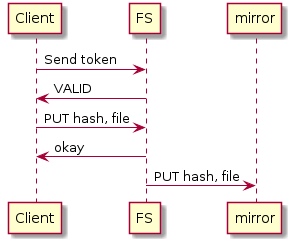
\includegraphics[width=.9\linewidth]{put_file.png}
\end{center}

\subsection{Case file server is dead}
\label{sec:org1f4a2df}
\begin{center}
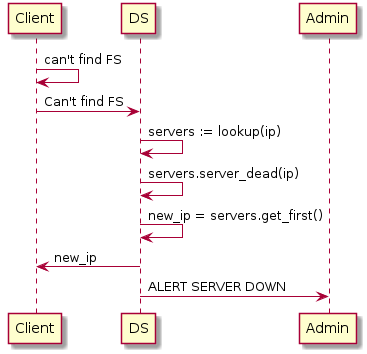
\includegraphics[width=.9\linewidth]{file_server_dies.png}
\end{center}

\section{Security}
\label{sec:org4eb9ee9}
Through TLS the main pillars of security are achieved
\begin{itemize}
\item Encryption
\item Authentication
\item Integrity
\end{itemize}

A careful admin can setup self sign certs in such a way as to guarantee this, in addition, it is very possible to add additional servers into this security model.

TLS allows us to use our simple but effective token protocol to auth users.

\subsection{The token}
\label{sec:org427503e}

A 3-tuple

$$ token := (t, c, exp) $$


Where:
\begin{itemize}
\item \(t := SHA256(urandom)\)
\item c := datetime.now()
\item exp := datetime.now + 1 week
\end{itemize}


The resulting token is encrypted under AS's private key1
\newline

t needs to be a quality random value, if anyone could predict it, they could forge a token and gain access.
\newline

related to this, it's also important that we encrypt under AS's priv key so that a fileserver can prove that the token was created by the AS.
\newline

c, and exp are self explanatory. A server knows that if the expiry date has been reached, not to accept the token. In addition a server might could be configured to not accept tokens of non realistic expirys.
e.g if a user got a token with expiry 5 years from now, a fileserver might want to reject. The extra value in the token just allows a bit of flexibility in the protocol in this regard. 

\section{Directory Service}
\label{sec:org64857a8}

\section{Replication}
\label{sec:org2576977}

\section{Caching}
\label{sec:orgdf28734}

\section{Transacctions}
\label{sec:org2a53f7c}

\section{Locking}
\label{sec:org87fe000}
\end{document}
